\newpage
\section{Auswertung}

    \subsection{Kontrastbestimmung}
        Die Messungen des Kontrasts ergeben, wie in Abbildung (Referenz) zu sehen, zwei Maxima im zu erwartenden Bereich von circa 45° und 135°.
        
        \FloatBarrier

        \begin{figure}[h]
          \centering
          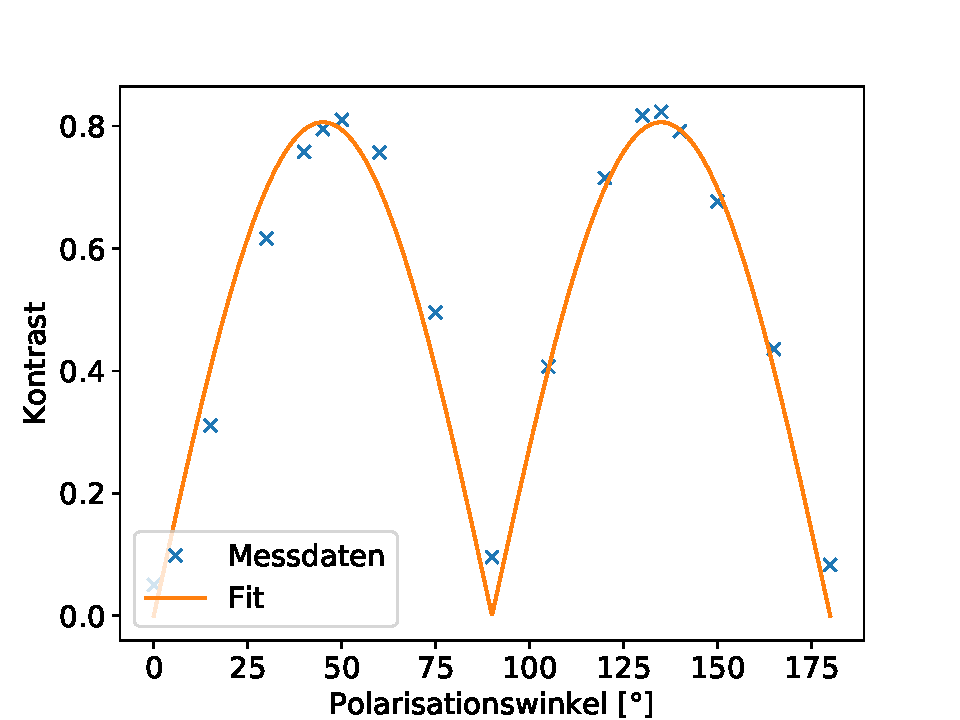
\includegraphics[width = 0.6\textwidth]{pictures/Kontrast.pdf}
          \caption{In der Grafik ist der gemessene Kontrast in Abhängigkeit des Polarisationswinkels des ins Interferometer einfallenden Lichtes aufgetragen.}
          \label{fig:Aufbau}
        \end{figure}

        \FloatBarrier

        Das absolute Maximum liegt mit \num{0.82} bei einem Polarisationswinkel von 135°, welcher demnach für die weiteren Messungen beibehalten wird.



    \subsection{Brechungsindex von Glas}
        Der Mittelwert der Nulldurchgänge aus den 10 aufgenommenen Messreihen (Referenz auf Tabelle) ergibt sich zu $\overline{\text{M}} = \num{33.40 +- 0.22}$ und entspricht auch dem Mittelwert der Maxima.
        Wenn $\overline{\text{M}}$ in Formel (Referenz zu Theorie) eingesetzt wird, lässt sich der Brechungsindex von Glas direkt berechnen:

        \begin{equation}
            \text{n}_{\text{Glas}} = \num{1.86 +- 0.01}
        \end{equation}


    \subsection{Brechungsindex von Luft}
        Bei den Messungen zur Bestimmung des Brechungsindizes von Luft, sind alle drei Messreihen exakt identisch, sodass sie nicht gemittelt werden müssen. Aus der Zahl der Maxima, die der Zahl der 
        Nulldurchgänge entspricht, lässt sich anhand von Formel (Referenz) und bekannten Parametern des Experiments, wie der Länge der Gaszelle und der Wellenlänge des Lasers, der zugehörige Brechungsindex
        bei entsprechendem Druck berechnen. Wenn diese Werte gegen den Druck in der Gaszelle aufgetragen werden ergibt sich ein linearer Zusammenhang, aus dem der Brechungsindex von Luft bei Normaldruck direkt 
        abgelesen werden könnte.

        \FloatBarrier

        \begin{figure}[h]
          \centering
          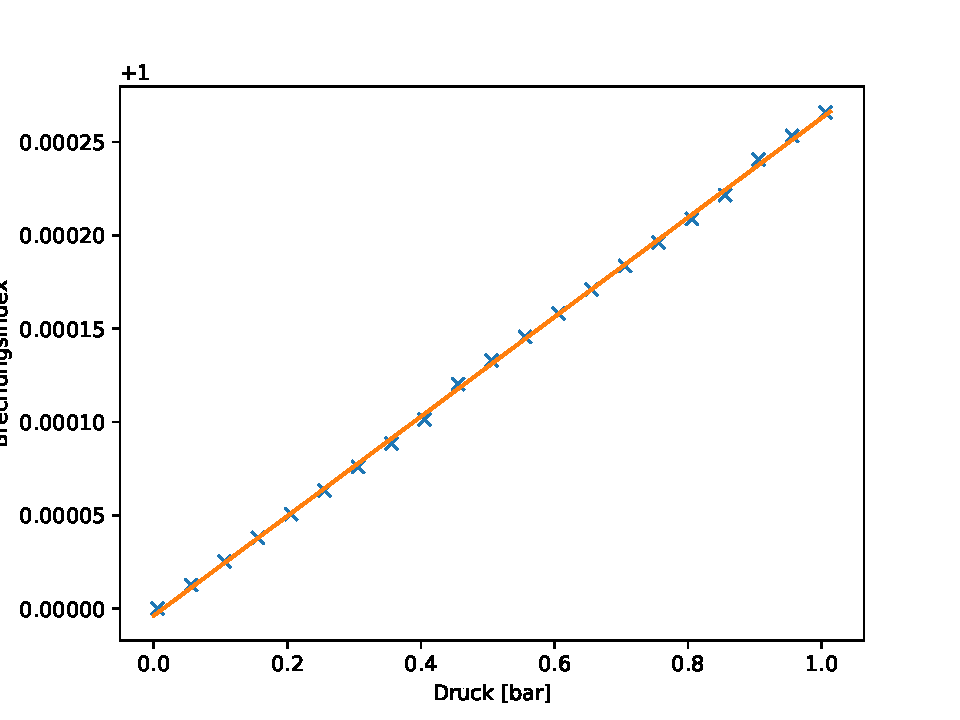
\includegraphics[width = 0.6\textwidth]{pictures/druck_lin.pdf}
          \caption{In der Grafik ist der lineare Zusammenhang zwischen dem Brechungsindex und dem Druck der Luft klar zu erkennen. Dieser wird auch mit folgenden Parametern gefitted: }
          \label{fig:Aufbau}
        \end{figure}

        \FloatBarrier

        In diesem Fall wird der Brechungsindex von Luft bei Normaldruck jedoch über das Lorentz-Lorenz-Gesetz bestimmt. Dazu muss zunächst die Molrefraktion bestimmt werden. Dieser ergibt sich
        über Formel (Referenz) wie folgt:

        \begin{equation}
            \text{A} = \num{0.4323 +- 0.0004} \qquad \text{bei} \qquad p = \SI{1006}{\milli\bar} 
        \end{equation}

        Mit der nun bekannten Molrefraktion A lässt sich der Brechungsindex von Luft bei Normalbedingungen direkt über das Lorentz-Lorenz-Gesetz (Referenz) bestimmen:

        \begin{equation}
            \text{n}_{\text{Luft}}(\SI{1013}{\milli\bar}, \, \SI{288.15}{\kelvin}) = \num{1.00027412 +- 0.00000027}     
        \end{equation}
        
